%%%%%%%%%%%%%%%%%%%%%%%%%%%%%%%%%%%%%%%%%%%%%%%%%%%%%%%%%%%%%%%%%%%%%%%%
\documentclass[twocolumn, prb, showpacs]{revtex4-1}
\usepackage{graphicx}
\usepackage{amsmath}
\usepackage{hyperref}
\usepackage{dcolumn}
\usepackage{xcolor}
\usepackage{caption}

\interfootnotelinepenalty=10000

\graphicspath{{./figures/}}

%\journal{International Journal of Hydrogen Energy}

%\bibliographystyle{elsarticle-num}

\newcommand{\note}[1]{\marginpar{\tiny\color{red}#1}}
\newcommand{\metal}{\mathcal{M}}
\newcommand{\molecule}{\mathcal{X}}
\begin{document}
%%%%%%%%%%%%%%%%%%%%%%%%%%%%%%%%%%%%%%%%%%%%%%%%%%%%%%%%%%%%%%%%%%%%%%%%




%%%%%%%%%%%%%%%%%%%%%%%%%%%%%%%%%%%%%%%%%%%%%%%%%%%%%%%%%%%%%%%%%%%%%%%%
%\begin{frontmatter}

\title{Understanding and improving hydrogen release in borohydrides
using additives: Beyond NH$_3$}


\author{D. Harrison}
\affiliation{Department of Physics, Wake Forest University,
Winston-Salem, NC 27109, USA.}


\author{T. Thonhauser}
\email{thonhauser@wfu.edu}
\affiliation{Department of Physics, Wake Forest University,
Winston-Salem, NC 27109, USA.}

\date{\today}


\begin{abstract}
An important aspect of successful hydrogen storage materials is their
hydrogen release mechanism, which---unfortunately---for many promising
materials occurs at impractical high or low temperatures.
In light of recent improvements observed when complexing borohydrides with NH$_3$, 
we performed an \emph{ab initio} investigation into the effects of complexing borohydrides
Al(BH$_4$)$_3$, Mg(BH$_4$)$_2$, and Zn(BH$_4$)$_2$ with new additive molecules CH$_4$, C$_2$H$_6$O,
and H$_2$O, as well as NH$_3$ as a benchmark. In order to find
candidate ground-state structures for these borohydride complexes,
we first performed an in-depth, evolutionary structure search.
These ground-state structures were then used to both evaluate their thermodynamic properties 
as well as investigate nearby metastable states that facilitate a favorable hydrogen release using the relatively new technique of
evolutionary metadynamics. We found that all of these additives markedly affect
(to varying degrees) the nearby metastable states relative to the unaltered
borohydride. In particular, complexing borohydrides with CH$_4$ and H$_2$O
results in particularly favorable properties for improving their hydrogen release.
Our study not only investigates new and promising hydrogen storage
materials, but also elucidates the hydrogen release mechanism in
processes difficult to experimentally characterize.
\end{abstract}


%\pacs{63.20.dk, 65.40.-b, 61.50.Ah, 88.30.rd}
% 63.20.dk      First-principles theory
% 65.40.-b      Thermal properties of crystalline solids
% 61.50.Ah      Theory of crystal structure, crystal symmetry;
%               calculations and modeling
% 88.30.rd      Inorganic metal hydrides



%%%%%%%%%%%%%%%%%%%%%%%%%%%%%%%%%%%%%%%%%%%%%%%%%%%%%%%%%%%%%%%%%%%%%%%%

%\end{frontmatter}

\maketitle


%%%%%%%%%%%%%%%%%%%%%%%%%%%%%%%%%%%%%%%%%%%%%%%%%%%%%%%%%%%%%%%%%%%%%%%%
\section{Introduction}\label{sec:introduction}
%%%%%%%%%%%%%%%%%%%%%%%%%%%%%%%%%%%%%%%%%%%%%%%%%%%%%%%%%%%%%%%%%%%%%%%%


Hydrogen has been identified as a promising alternative to fossil fuels due to
its potential to be a clean, renewable energy carrier
\cite{Kunowsky_2013:material_demands, Durbin_2013:review_hydrogen,
Crabtree_2004:hydrogen_economy}. However, in its natural state, hydrogen has an
unsuitably low volumetric density for automotive applications, leading to much
research on more effective hydrogen storage methods
\cite{Harrison_2015:materials_hydrogen,Ahluwalia_2012:on-board_off-board}, with
clear goals outlined by the Department on Energy (DOE)
\cite{Yang_2010:high_capacity, DOE_Targets_Onboard_2009}. Borohydrides are a
class of complex hydrides which are of particular interest due to their high gravimetric
and volumetric densities, although they typically suffer from hydrogen
desorption temperatures over 85~$^\circ$C, i.e.\ the maximum delivery
temperature set by the DOE for fuel cell operation in vehicles
\cite{Yang_2010:high_capacity, Graetz_2009:new_approaches,
Ronnebro_2011:development_group, Li_2011:recent_progress,
Rude_2011:tailoring_properties,
Jain_2010:novel_hydrogen,Orimo_2007:complex_hydrides,Umegaki_2009:boron-_nitrogen-based,George_2010:structural_stability}.

Various methods have been used in order to improve the properties of various
borohydrides, including destabilizing via reactions with other hydrides
\cite{Vajo_2005:reversible_storage, Alapati_2007:using_first,
Alapati_2008:large-scale_screening, Li_2008:dehydriding_rehydriding}, alloying
\cite{Nickels_2008:tuning_decomposition,Li_2007:materials_designing,Lee_2010:effect_mg},
cation substitution \cite{Setten_2007:ab_initio}, anion substitution
\cite{Brinks_2008:adjustment_stability}, and adding catalysts
\cite{Li_2007:effects_ball}.  In general, the goal of most of these methods is
to lower the hydrogen desorption temperature by altering either the kinetics or
thermodynamics of the reaction.  One particularly successful method is the complexing of borohydrides with additional molecules such as
ammonia (NH$_3$) \cite{Chu_2010:structure_hydrogen, Gu_2012:structure_decomposition, Jepsen_2014:boron-nitrogen_based,
Roedern_2015:ammine-stabilized_transition-metal, Sun_2012:new_ammine, Yuan_2012:structure_hydrogenstorage, Welchman_2017:decomposition_mechanisms}.
The effect of introducing ammonia into borohydrides depends somewhat on the
particular borohydride, but the effects are almost always beneficial.  For
borohydrides which are too stable (i.e.\ the temperature at which they release
hydrogen is too high), ammonia complexing has been found to decrease the
hydrogen release temperature remarkably; for borohydrides which are too
unstable (i.e.\ the temperature at which they release
hydrogen is too low) ammonia complexing has been found to increase the
temperature through a mechanism we have recently uncovered
\cite{Welchman_2017:decomposition_mechanisms}.

Because of the beneficial effects of ammonia complexing in borohydrides,
in this work we investigate
the effects of complexing borohydrides with other small molecules. In particular, we
investigate the effects of complexing Al(BH$_4$)$_3$, Mg(BH$_4$)$_2$, and
Zn(BH$_4$)$_2$ with H$_2$O, CH$_4$, C$_2$H$_6$O, and NH$_3$. These borohydrides were
chosen so as to have a representative range of stabilities and structures out
of the class of borohydrides \cite{Nakamori_2007:thermodynamical_stabilities} and the small molecules were chosen so as to have a
range of polarity and size. We included NH$_3$ in our study as a benchmark
for which a myriad of experimental data exists \cite{Chu_2010:structure_hydrogen, Gu_2012:structure_decomposition, Jepsen_2014:boron-nitrogen_based,
Roedern_2015:ammine-stabilized_transition-metal, Sun_2012:new_ammine, Yuan_2012:structure_hydrogenstorage}.

To fully capture the effects of complexing borohydrides, the thermodynamics and
kinetics of the resulting phases has to be investigated. While the former is
fairly straightforward within \emph{ab initio} materials modeling, the latter
is almost prohibitively complex. Although basic transition-state search algorithms
exist that can in principle find kinetic barriers \cite{Henkelman_2000:climbing_image,
Henkelman_2000:improved_tangent}, the problem is that 
even in simple borohydrides the release mechanism is too complicated, typically
forming a B$_{12}$H$_{12}$ intermediate after several steps \cite{Yan_2011:formation_process}.
For this same reason, while \emph{ab initio}
molecular dynamics (MD) could theoretically be employed to study the hydrogen release process,
practically speaking the large energy barrier to this process causes the required MD time scale to be far beyond reach.
There are a number of strategies for dealing with this situation which are typically referred to as
umbrella sampling. Of pertinence to this study is metadynamics, a technique 
to sample rare events by adding cumulative Gaussian energy
penalties to regions of phase space that have already been explored. This technique
provides a means to sample rare events within systems
which otherwise would be unobservable due to their
large activation energy.
A recent and relatively unknown innovation to this technique is known as \emph{evolutionary metadynamics} \cite{Zhu_2012:evolutionary_metadynamics, Zhu_2015:generalized_evolutionary}; a discussion of this
method (and our implementation of it) is given in the ``Appendix'' section
of this paper. 
In our study, we have used this novel technique to
investigate nearby metastable states and the effect of complexing
on them to deduce valuable hydrogen release characteristics. In conjunction with
the Bell--Evans--Polanyi principle of physical chemistry 
\cite{Bell_1936:theory_reactions,Evans_1936:further_considerations}---wherein the activation energy for
a reaction can be approximated by the enthalpy of reaction---we obtain
crucial insights into both the mechanisms and approximate kinetic barriers for the initial
steps in the borohydride decomposition, including the effect
that additive molecules have upon these steps. 








%%%%%%%%%%%%%%%%%%%%%%%%%%%%%%%%%%%%%%%%%%%%%%%%%%%%%%%%%%%%%%%%%%%%%%%%
\section{Computational Details}
%%%%%%%%%%%%%%%%%%%%%%%%%%%%%%%%%%%%%%%%%%%%%%%%%%%%%%%%%%%%%%%%%%%%%%%%

%%%%%%%%%%%%%%%%%%%%%%%%%%%%%%%%%%%%%%%%%%%%%%%%%%%%%%%%%%%%%%%%%%%%%%%%
\subsection{\emph{Ab Initio} Ground-State Calculations}

We performed {\it ab initio} simulations at the 
density functional theory (DFT) level as implemented in \textsc{Vasp}
\cite{Kresse_1996:efficient_iterative, Kresse_1999:ultrasoft_pseudopotentials},
using the standard projector augmented wave (PAW) pseudopotentials provided. A plane wave energy cutoff
of 520~eV and k-point mesh density of
0.08~\AA$^{-1}$ were used unless otherwise noted. Energy convergence
criterion and force criterion were varied depending on the level of accuracy desired
for the method employed, with specific details outlined in the corresponding sections below.
As previous studies on borohydrides found that van der Waals interactions are
crucial to accurately model these materials due to weak interactions among the
BH$_4$ units \cite{Miwa_2007:first-principles_study,
Lodziana_2010:multivalent_metal, Bil_2011:van_waals}, we employed the exchange-correlation functional vdW-DF
\cite{Thonhauser_2015:spin_signature, Berland_2015:van_waals,
Thonhauser_2007:van_waals, Langreth_2009:density_functional}, which includes a
truly non-local correlation term to capture van der Waals binding.

%As an overview, less stringent parameters were utilized for most of the structure search
%run, while the best structures found via the structure search were treated
%to tighter convergence. All structures used to calculate thermodynamic results
%were treated to a very high level of convergence, while calculations on metastable
%structures were subject to a medium level of convergence.








%%%%%%%%%%%%%%%%%%%%%%%%%%%%%%%%%%%%%%%%%%%%%%%%%%%%%%%%%%%%%%%%%%%%%%%%
\subsection{Structure Searches}

In order to study borohydrides with additive molecules, it was first necessary
to determine the corresponding ground-state structures. To this end, we used the crystal structure
prediction program \textsc{Uspex} \cite{Oganov_2006:crystal_structure,
Oganov_2011:how_evolutionary, Lyakhov_2013:new_developments,
Zhu_2012:constrained_evolutionary} in combination with \textsc{Vasp}.
\textsc{Uspex} was configured to run a three-dimensional
molecular structure search with a population size of 10 at each generation. The
structure search was stopped if the same structure had the lowest energy for 6
generations in a row or if a total of 30 generations were ran. Three molecules
were used in each structure search: the borohydride molecule, the borohydride
metal, and the additive molecule; one formula unit was used for both the
borohydride and the additive molecule. For example, for the
complexed Al(BH$_4$)$_3$$\cdot$NH$_3$ structure, a molecular structure search was performed
with 1~Al, 1~NH$_3$ molecule, and 3 BH$_4$ molecules. The relaxations in the structure search were done
in \textsc{Vasp}, using the conjugate-gradient method with an electronic convergence of $10^{-4}$~eV for 100 ionic
steps, with the unit cell fully allowed to relax.




%%%%%%%%%%%%%%%%%%%%%%%%%%%%%%%%%%%%%%%%%%%%%%%%%%%%%%%%%%%%%%%%%%%%%%%%
\subsection{Ground-State Starting Structures}


We then took the best structures from each structure search and further
relaxed them in \textsc{Vasp}, using an electronic
convergence of $10^{-7}$~eV until all forces were less than $10^{-3}$~eV/\AA.
In addition, the energies of the elements, additive molecules, and pure borohydrides were calculated using the
same criteria. For those elements or molecules which exist in the gaseous
phase under standard conditions (e.g.\ H$_2$), a $10\times10\times10$~\AA\ box was used.  From this, we
then computed thermodynamic properties of these structures, finding
both their enthalpy of formation and the enthalpy of reaction to form the
borohydride complex from the borohydride molecules and the additive molecules.
Note that the most stringent criteria was used for this stage of the study
(i.e.\ relaxing ground-state starting structures) not only because it was
important to have accurate structures in order to calculate the thermodynamic
properties, but because these structures formed the basis for all of the
future work studying their metastable states.
From our previous study on borohydrides we know that
vibrational contributions to the relative differences in
formation enthalpy are negligible (e.g.\ the zero-point energy contribution
is $\sim$40~kJ/mol~BH$_4$ regardless of the metal for Mg, Zn, Al, and Sc borohydrides)
\cite{Harrison_2014:tuning_hydrogen,Harrison_2016:suppressing_diborane}, so those effects
were not included in the present study.

For the pure borohydride structures, we did not perform a structure search,
as their ground state structures were already known, but instead used
the listed known structures.
The structure used for Al(BH$_4$)$_3$ was the
solid-phase $\beta$-Al(BH$_4$)$_3$ taken from the theoretical work of Miwa et
al.\
\cite{Miwa_2007:first-principles_study,Aldridge_1997:some_tetrahydroborate},
the structure for Zn(BH$_4$)$_2$ was taken from Nakamori et al.\
\cite{Nakamori_2006:correlation_between}, the structure for boron was the 106
atom $\beta$-rhombohedral structure suggested by van Setten et
al.~\cite{Setten_2007:thermodynamic_stability}, and the structure used for
Mg(BH$_4$)$_2$ was the 99 atom structure found to be nearly isoenergetic
to the true ground state structure (which was not used due to its large unit
cell with 330 atoms) \cite{Bil_2011:van_waals}. 




%%%%%%%%%%%%%%%%%%%%%%%%%%%%%%%%%%%%%%%%%%%%%%%%%%%%%%%%%%%%%%%%%%%%%%%%
\subsection{Metastable Structures}

In order to generate a host of metastable structures, we again used
\textsc{Uspex} in conjunction with \textsc{Vasp}, although this time utilizing
the evolutionary metadynamics method \cite{Zhu_2012:evolutionary_metadynamics, Zhu_2015:generalized_evolutionary}. 
For the borohydride-additive structures, the initial structures used were $2\times2\times2$ supercells
(such that each structure had 8 formula units)
created from each of the best structures found from the initial structure search
(which were subsequently further relaxed as described in the previous section); supercells
were created for these structures in order to lessen interactions among periodic images when
the structure is perturbed. No supercells were created for the pure borohydride structures
as they already contained several formula units per unit cell. At each
generation, a population size of 10 structures was used. The Gaussian penalty height
and width used were 16\,000 \AA$^{3}$~kbar and 1.6 \AA. At each generation, a two-stage relaxation was performed.
First, all of the structures within the generation were relaxed using the
conjugate-gradient method with an energy cutoff of 415~eV and an electronic
convergence of $10^{-3}$~eV until all forces were less than 0.3~eV/\AA. This
step was done without varying the unit cell size and shape. After this step,
the best structures were chosen for a subsequent relaxation, where cell size
and shape were allowed to vary and tighter parameters were used: the structures
were relaxed using the conjugate-gradient method with an electronic convergence
of $10^{-5}$~eV until all forces were less
than 0.1~eV/\AA. Due to the large unit cell sizes and computational speed needed, 
a single k-point was used for all metastable structure calculations. For each structure, at least 8 generations were performed.
 
The best structures from each generation---i.e.\ the structures that underwent
full cell shape and size relaxation---were then analyzed as presented in Section~\ref{sec:metadynamics}. For future
analysis, it was desirable to create a list of molecules for each structure. This was done according to the following guidelines:
Any atoms within 1.6~\AA\ of each other
were considered to be bonded, and a molecule was considered to be a collection
of atoms where each member is bonded to at least one other member in the
collection. One exception was for a hydrogen-hydrogen interaction, which were
considered to be bonded if they were within 1~\AA\ of each other. These criteria work well 
for the bonds we were interested in, namely stronger bonds involving B, C, H, N, and O, due to their
covalent radii being approximately 0.8~\AA\ or less. It should be noted (and will become apparent in the discussion of results) that, as the metal
atoms (Mg, Al, and Zn) tend to have significantly larger radii, we are implicitly neglecting them in our analysis, and instead
focusing on the borohydride complexes and additive molecules.








%%%%%%%%%%%%%%%%%%%%%%%%%%%%%%%%%%%%%%%%%%%%%%%%%%%%%%%%%%%%%%%%%%%%%%%%
\section{Thermodynamics Results of Complexing Borohydrides}
%%%%%%%%%%%%%%%%%%%%%%%%%%%%%%%%%%%%%%%%%%%%%%%%%%%%%%%%%%%%%%%%%%%%%%%%

As the first step in our investigation of the effect of complexing
borohydrides, we compute their thermodynamical properties. 
Table~\ref{tab:formation_enthalpies} shows the formation enthalpies for all borohydride-additive
combinations, including no additive, in units of kJ/mol~BH$_4$. As a reminder, recall that there is one formula unit
of additive molecule per formula unit of the metal borohydride. 
Overall,
these results confirm that all
of the structures studied are stable with respect to decomposition to elements.
It also becomes immediately clear that adding the additives in all cases
increases the stability of the materials.

More interestingly, we recently developed a criterion for determining
whether or not a borohydride will produce diborane---an undesirable byproduct that is poisonous to the fuel cell---upon decomposition, based on the formation enthalpy of
the borohydride \cite{Harrison_2016:suppressing_diborane}. In particular, we showed that
for values greater than $\sim-110$~kJ/mol~BH$_4$ diborane will be produced; while
this criterium was developed in the context of pure borohydrides, there is
evidence which suggests if may be more generally applicable \cite{Harrison_2016:suppressing_diborane,Gu_2012:structure_decomposition}. 
We thus predict that all additives
to some degree suppress diborane production during the hydrogen release (albeit not necessarily reaching the $-$110~kJ/mol~	BH$_4$ threshold under the additive conentration studied), with H$_2$O and
C$_2$H$_6$O providing the greatest degree of suppression.


\begin{table}
\caption{\label{tab:formation_enthalpies}Formation enthalpies $\Delta
H_f$ in kJ/mol~BH$_4$ for Al(BH$_4$)$_3$, Mg(BH$_4$)$_2$, and Zn(BH$_4$)$_2$
complexed with various different additives.}
\begin{tabular*}{\columnwidth}{@{}l@{\extracolsep{\fill}}rrrrr@{}}\hline\hline
                & \multicolumn{5}{c}{Additives}\\[1ex]
                & None        & NH$_3$     & CH$_4$     & C$_2$H$_6$O & H$_2$O     \\\hline
Al(BH$_4$)$_3$  &  $-56.54$   & $-114.71$  & $-93.99$   & $-194.33$   & $-175.58$  \\
Mg(BH$_4$)$_2$  &  $-131.20$  & $-192.48$  & $-175.51$  & $-317.23$   & $-294.42$  \\
Zn(BH$_4$)$_2$  &  $-16.69$   & $-98.50$   & $-69.63$   & $-209.58$   & $-185.10$  \\\hline\hline
\end{tabular*}
\end{table}


To further investigate the stability of borohydride-additive combinations,
we also calculate the energy gained from combining the borohydride and its additive,
i.e.\ the reaction enthalpy to form the complexed borohydride
%
\begin{equation}
\metal\,({\rm BH}_4)_n + \molecule \;\;\longrightarrow\;\;
\metal\,({\rm BH}_4)_n \cdot \molecule
\end{equation}
%
for the various combinations of metals $\metal$ and additives $\molecule$.
The results depicted in Fig.~\ref{fig:reaction_enthalpies} reveal two clear trends:
(i) The NH$_3$, C$_2$H$_6$O, and H$_2$O additives result in very stable
compounds, whereas CH$_4$ produces less stable complexed borohydrides. The obvious and most likely
explanation for this result is the polarity of the additives: the polarity of NH$_3$, C$_2$H$_6$O, and H$_2$O
enable them to bind stronger with the anions and cations in the borohydride than with the 
nonpolar CH$_4$.
Of note, when CH$_4$ is combined with Mg(BH$_4)_2$, the overall
compound is predicted to be slightly unstable with respect to phase-segregation,
although not so much so that the phase could not be stabilized kinetically or due to the entropy of mixing.
(ii) The relative stability of an additive is inversely proportional to the stability of the
borohydride, a trend that we will again see in the discussion of the metadynamics
results. By this we mean that, as seen by referencing Table~\ref{tab:formation_enthalpies}, the least
stable borohydrides (e.g.\ Zn(BH$_4$)$_2$) have the strongest affinity for additive molecules.

\begin{figure}
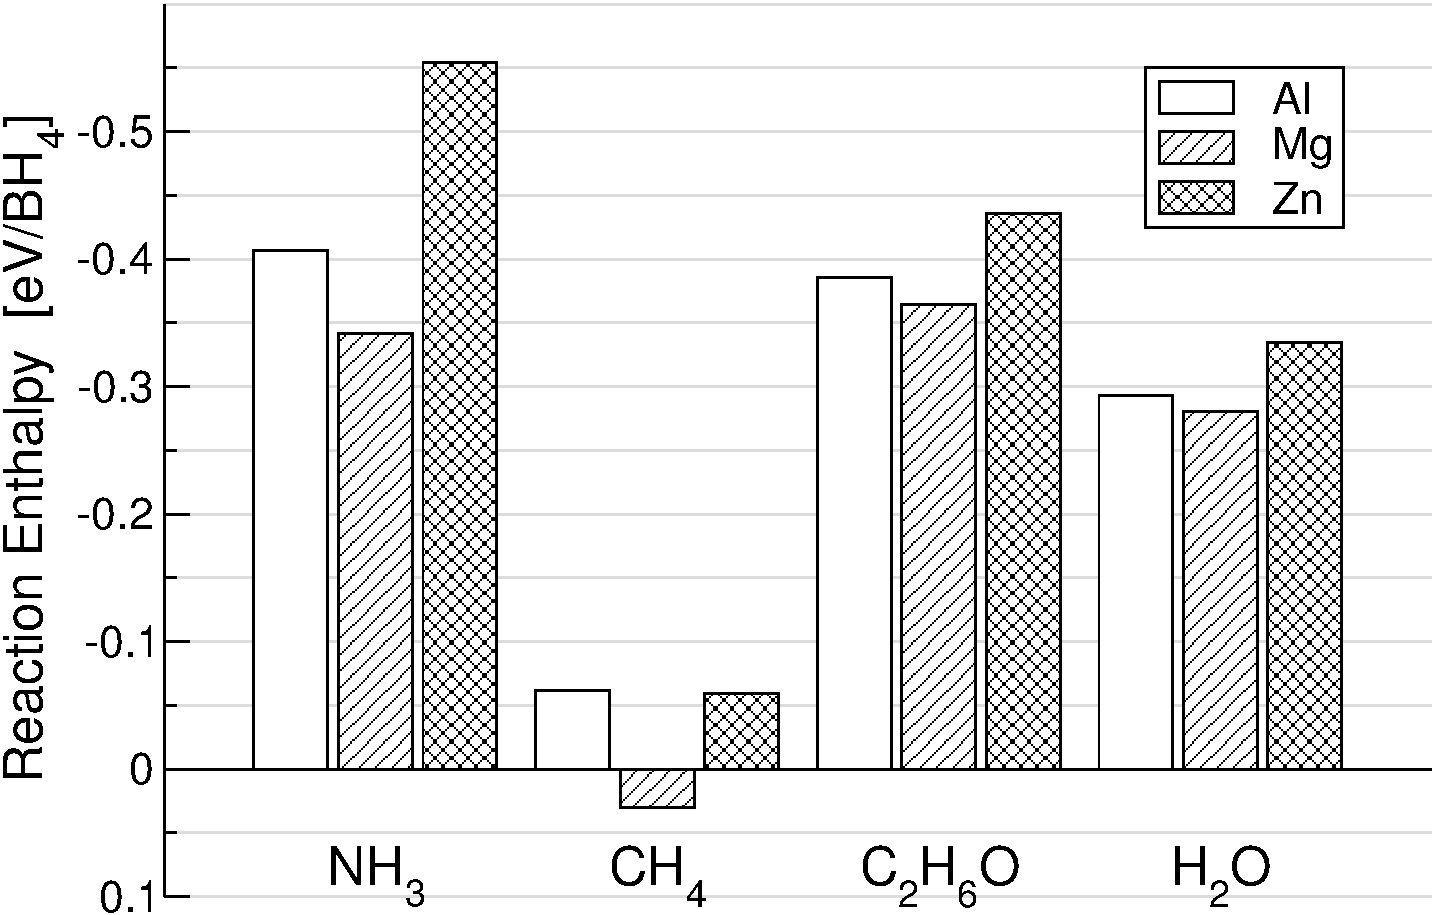
\includegraphics[width=\columnwidth]{reaction_enthalpy}
\caption{\label{fig:reaction_enthalpies}Reaction enthalpy to form the
complexed borohydride, i.e.\ $\metal\,($BH$_4)_n + \molecule\rightarrow
\metal\,($BH$_4)_n \cdot \molecule$ for $\metal$ = Al, Mg, Zn and
$\molecule$ = NH$_3$, CH$_4$, C$_2$H$_6$O, H$_2$O. Negative values
indicate a favorable reaction.}
\end{figure}








%%%%%%%%%%%%%%%%%%%%%%%%%%%%%%%%%%%%%%%%%%%%%%%%%%%%%%%%%%%%%%%%%%%%%%%%
\section{Metadynamics Results of Complexing Borohydrides}
%%%%%%%%%%%%%%%%%%%%%%%%%%%%%%%%%%%%%%%%%%%%%%%%%%%%%%%%%%%%%%%%%%%%%%%%


%%%%%%%%%%%%%%%%%%%%%%%%%%%%%%%%%%%%%%%%%%%%%%%%%%%%%%%%%%%%%%%%%%%%%%%%
\subsection{The Idea and Implicit Assumptions Behind Metadynamics}

Starting from a suitable collection of accurate structures both for pure borohydrides and borohydride complexes, evolutionary metadynamics allows
us to take these structures as input and catalog the energy and composition of a large number of nearby metastable states for these structures as output. Our goal in doing this is
to study the first critical steps in the decomposition of a borohydride and use these to help us understand what relation there is (if any) between these
first steps and the full decomposition (by comparing to known experimental results), as well as determine the effects additives have on these initial
decomposition steps. 

As an example, it is known that complexing Mg(BH$_4$)$_2$ with NH$_3$ decreases the temperature of hydrogen release \cite{Soloveichik_2008:ammine_magnesium}.
We would expect that this phenomenon is liekly due to NH$_3$ somehow lowering the energy barrier for hydrogen production. To see this, we would look at the energy
of resultant metastable structures which contain H$_2$ molecules for pure Mg(BH$_4$)$_2$ and compare that to the energy of resultant metastable structures which
contain H$_2$ molecules for Mg(BH$_4$)$_2$$\cdot$NH$_3$. In fact, as will be seen in the subsequent discussion, that is exactly what we find.

Before continuing, this is a good opportunity to discuss an implicit assumption that we
are making in discussing these results: that the energy difference between states
is approximately equal to the energy barrier to transition between those states
(i.e.\ the Bell--Evans--Polanyi principle). We believe this assumption to be reasonable
partially based on the methodology of evolutionary metadynamics, which finds states
nearby in phase-space to the initial provided ground-state structure. However,
we further support this assumption by comparing to previous nudged elastic band (NEB)
calculations on diborane production in borohydrides: through discussion with one of the authors
studying these reaction barriers we learned that the energy difference between the transition-state
structure and the final metastable structure to be rather small in comparison to the total energy barrier ($\sim$0.15~eV, whereas the total
barrier is typically $\sim$1.35~eV).\cite{Welchman_2017:decomposition_mechanisms} Given this, throughout our discussion we will often treat the
energy differences between our structures as the energy barrier to transition between those structures,
while in reality this is an approximation.

This is also a good point to remind the reader that, while in our study we have
investigated nearby metastable states to the ground structures of borohydrides
and borohydride-additive complexes, the full decomposition reaction includes several
additional steps which include both further decomposition of the structure and
the diffusion of hydrogen (and possibly other gases, such as diborane) from the
bulk material. Our implicit assumption in comparing our metadynamics results to experimental
results is that the initial steps in the decomposition reaction directly affects the full
decomposition. This would be the case e.g.\ if the initial steps are the rate-limiting steps in the reaction. 
In other words, while the exact processes and barriers for the full decomposition reactions remain a mystery,
the fact that there is good agreement between our metadynamics results and experimental data
seems to suggest that the initial decomposition reaction steps (as approximated by our investigation
into nearby metastable states) are critical to some degree for determining the pathway
for the full decomposition pathway.


%%%%%%%%%%%%%%%%%%%%%%%%%%%%%%%%%%%%%%%%%%%%%%%%%%%%%%%%%%%%%%%%%%%%%%%%
\subsection{Metadynamics on Al(BH$_4)_3\cdot$NH$_3$ as an Example}



Figure~\ref{fig:example_plot} shows, as an example, a plot of relative
stability vs.\ H$_2$ concentration for the best structures produced by USPEX
from the evolutionary metadynamics simulation for the structure
Al(BH$_4$)$_3\cdot$NH$_3$. The y-axis is defined simply as the energy of these
structures in eV/BH$_4$ unit while the x-axis is defined as the number of hydrogens in
hydrogen molecules divided by the total number of hydrogens originally
contained in the BH$_4$ molecules (e.g. for a $2\times2\times2$ supercell of
Al(BH$_4$)$_3$$\cdot$NH$_3$, i.e.\ 8 formula units, 8~H$_2$ molecules would have a relative H$_2$
concentration of 16.67\%, as there are 96 total hydrogens in the 24 BH$_4$ units). Note that using this definition
it is possible, for structures containing additives, to have a relative H$_2$ concentration above 100\%.


\begin{figure}
\begin{center}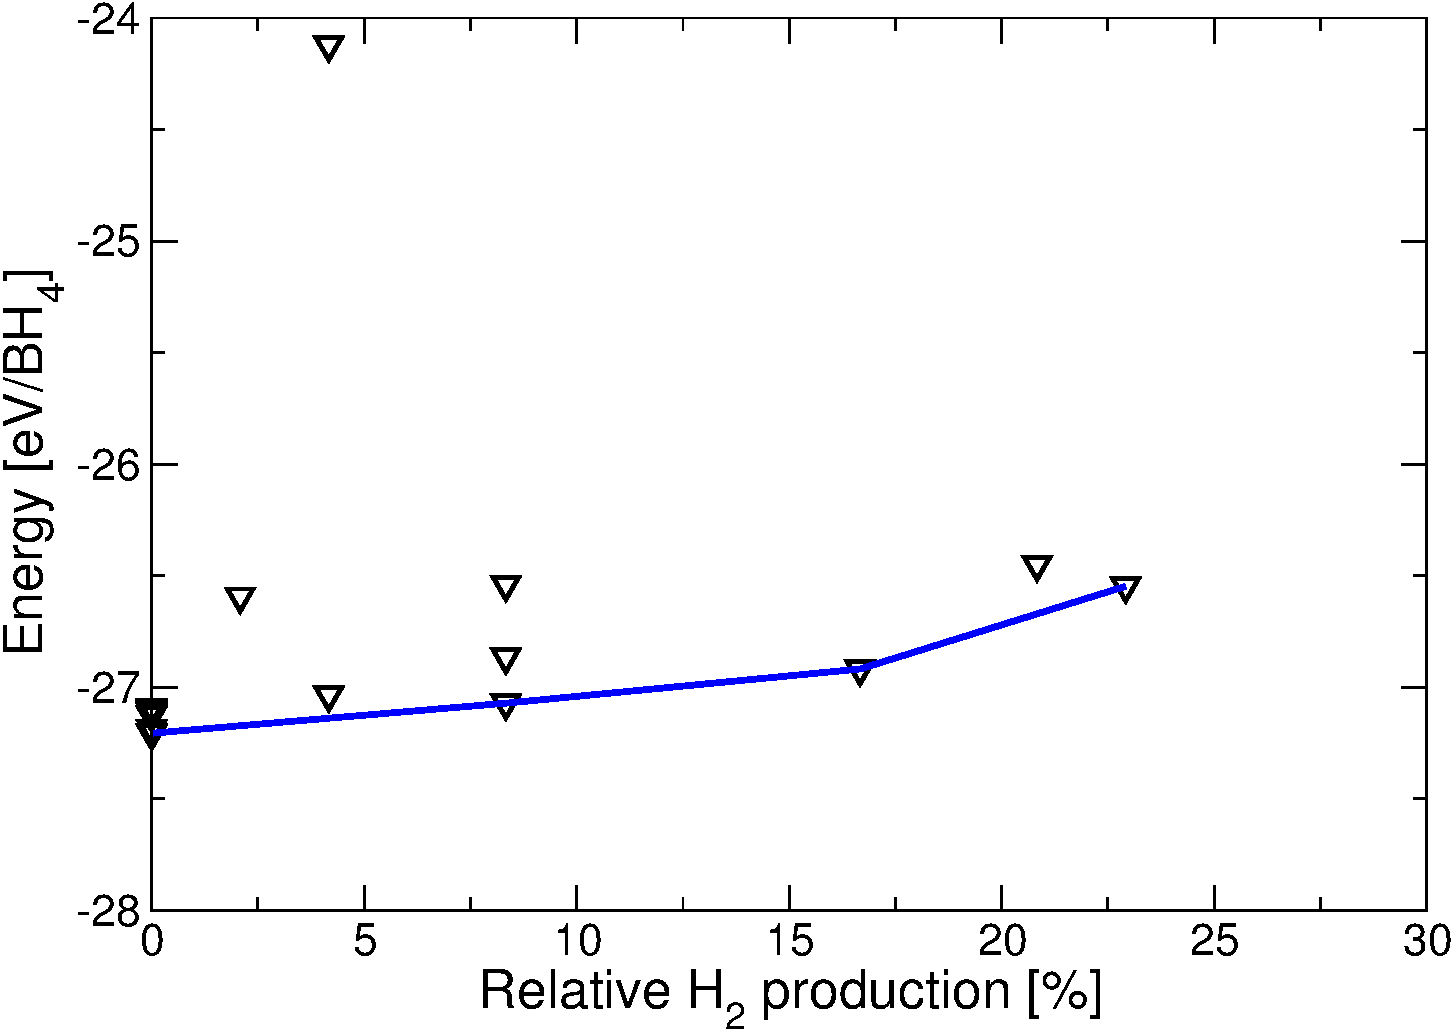
\includegraphics[width=0.85\columnwidth]{example1}\end{center}
\caption{\label{fig:example_plot}Example plot showing energy vs.\ relative H$_2$ concentration for
the best structures at each generation found by the evolutionary metadynamics structure search
for Al(BH$_4)_3\cdot$NH$_3$. The blue line represents the bottom part of the convex hull, illustrating
the technique used to develop all of the later plots.}
\end{figure}


As an aside to give perspective on the data itself (not just for this example but for all combinations of borohydride and additive studied), in total 1448 structures were generated among all 12 combinations of borohydride and additive. The points shown in Fig.~\ref{fig:example_plot}
are the 17 best structures out of 83 total structures produced over 8 generations specifically for Al(BH$_4)_3\cdot$NH$_3$ (at each generation,
USPEX records at least one best structure, although typically around 2, leading to 17 structures from 8 generations). Of these 17 structures plotted, 8 of these structures
have 0 relative H$_2$ concentration, and, at least in terms of molecular composition, are nearly 
identical to the initial starting structure. Conceptually, when a structure is perturbed along
a given direction (e.g.\ given by a soft eigenmode) and then relaxed, if the perturbation
isn't sufficiently large the system simply reverts to a state nearly identical to its unperturbed
state. As metadynamics naturally induces stronger perturbations in later generations (as the Gaussian
energy penalty has been allowed to accumulate), it is more likely to observe system states dissimilar to the
ground-state structure. Similarly for this reason, in systems with relatively high-energy metastable states,
it often takes several generations to observe structures notably dissimilar to the initial ground-state structure.

Looking at the spread of the points, it's clear that near a given hydrogen
concentration range there are a variety of metastable states with a relatively large
range in energy; from our observations, this range in energy can be due to a
variety of structural changes, including differences in volume, molecule
composition (e.g.\ one structure may have more BH$_3$ and BH$_5$ units than
another), or simply various differences in molecule positions. However, our
interest was looking at the most stable structure at any given hydrogen
concentration, with our assumption being that in order to produce this amount
of hydrogen going through this state would represent the most favorable
pathway, as per the Bell-Evans-Polanyi principle we would also expect this to be the
most favorable pathway kinetically.

Because our primary interest was the structures which produced H$_2$, and
furthermore only the most energetically favorable ones, we decided to restrict
ourselves to looking at the bottom half of the convex hull for all of the
metastable structures, as shown as an example for Al(BH$_4)_3\cdot$NH$_3$ in Fig.~\ref{fig:example_plot}.

%%%%%%%%%%%%%%%%%%%%%%%%%%%%%%%%%%%%%%%%%%%%%%%%%%%%%%%%%%%%%%%%%%%%%%%%
\subsection{Metadynamics Analysis of Complexing Borohydrides}
\label{sec:metadynamics}

\subsubsection{Overview}

Doing this for all combinations of borohydrides and additives, we were able to
get an estimate for the energetic cost of hydrogen production for all of the
possible combinations studied. Plotted in Fig.~\ref{fig:main_plot} are all of
structures which form the aforementioned bottom half of the convex hull for all
additives studied for a given borohydride. The y-axis is once again the energy
of the structure per BH$_4$, but all plots have been shifted so that the initial
structure of each is defined to have an energy of 0. This way, the relative
cost of forming hydrogen among different additives could be compared.


\begin{figure}
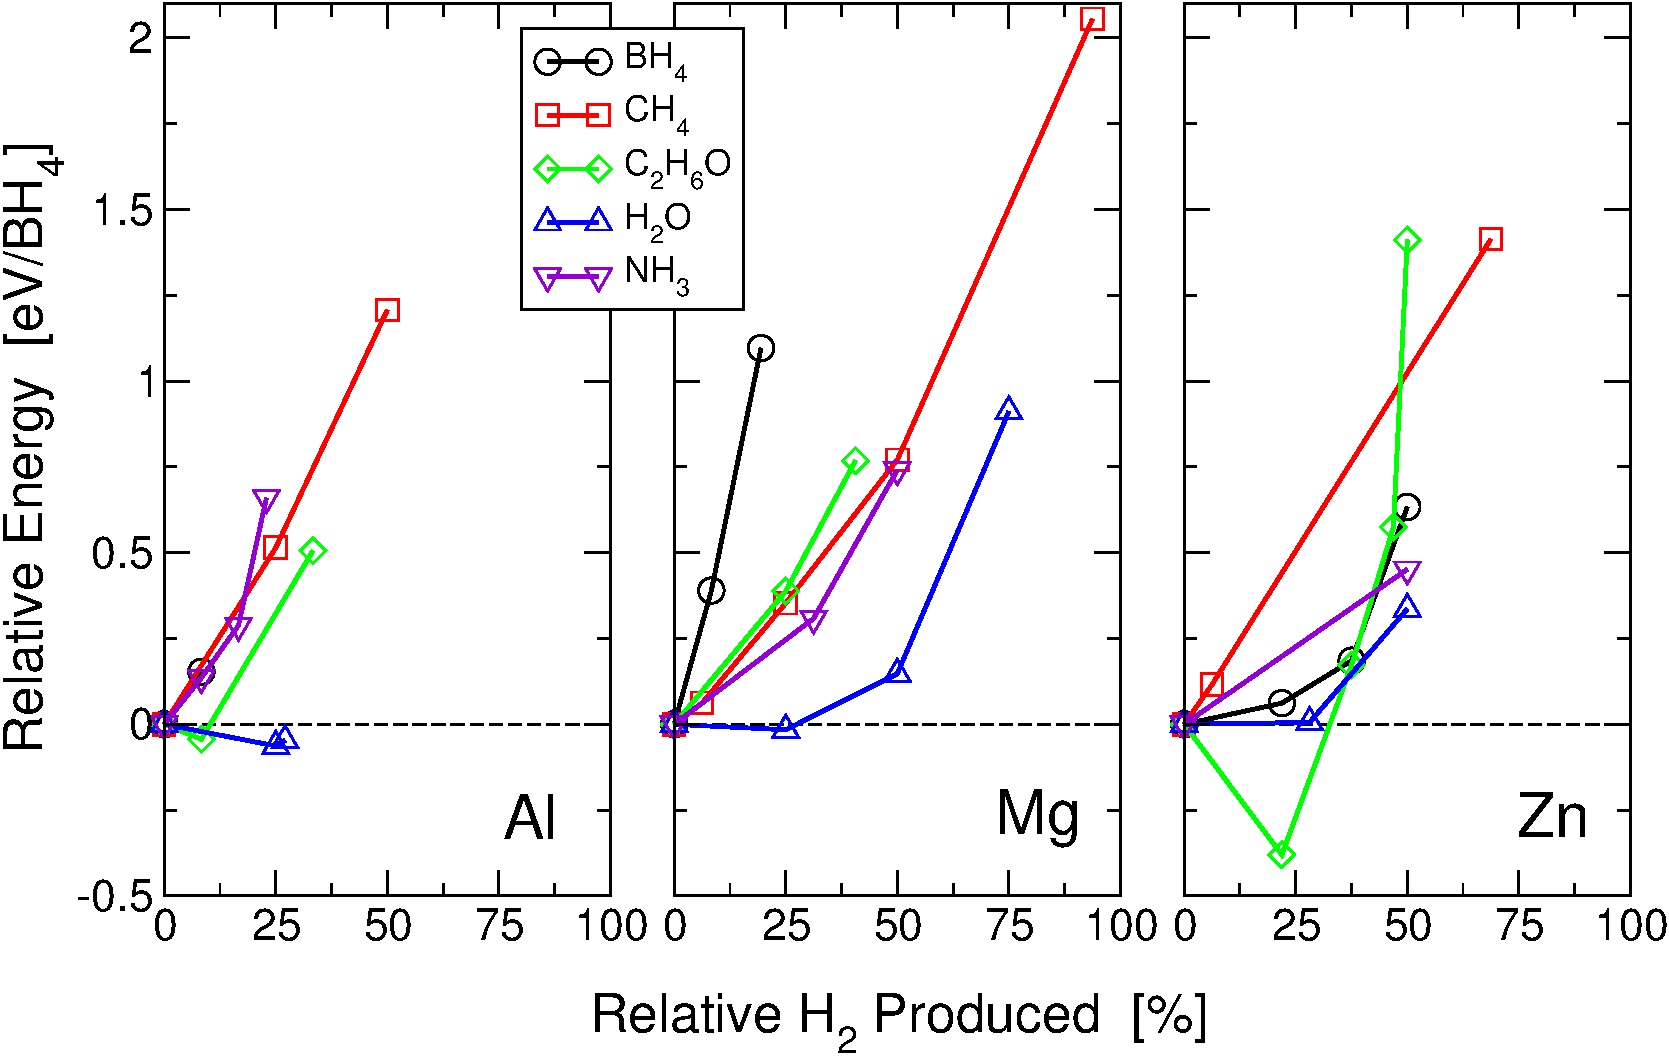
\includegraphics[width=\columnwidth]{H2_production}
\caption{\label{fig:main_plot}Plot of energy vs.\ relative H$_2$ production for all structures
found in structure search
lying along the bottom hull for Al(BH$_4$)$_3$, Mg(BH$_4$)$_2$, and Zn(BH$_4$)$_2$, and their corresponding additive molecules. `BH$_4$' on the plot legend indicates the pure
borohydride, i.e.\ no additive.}
\end{figure}


\begin{figure}
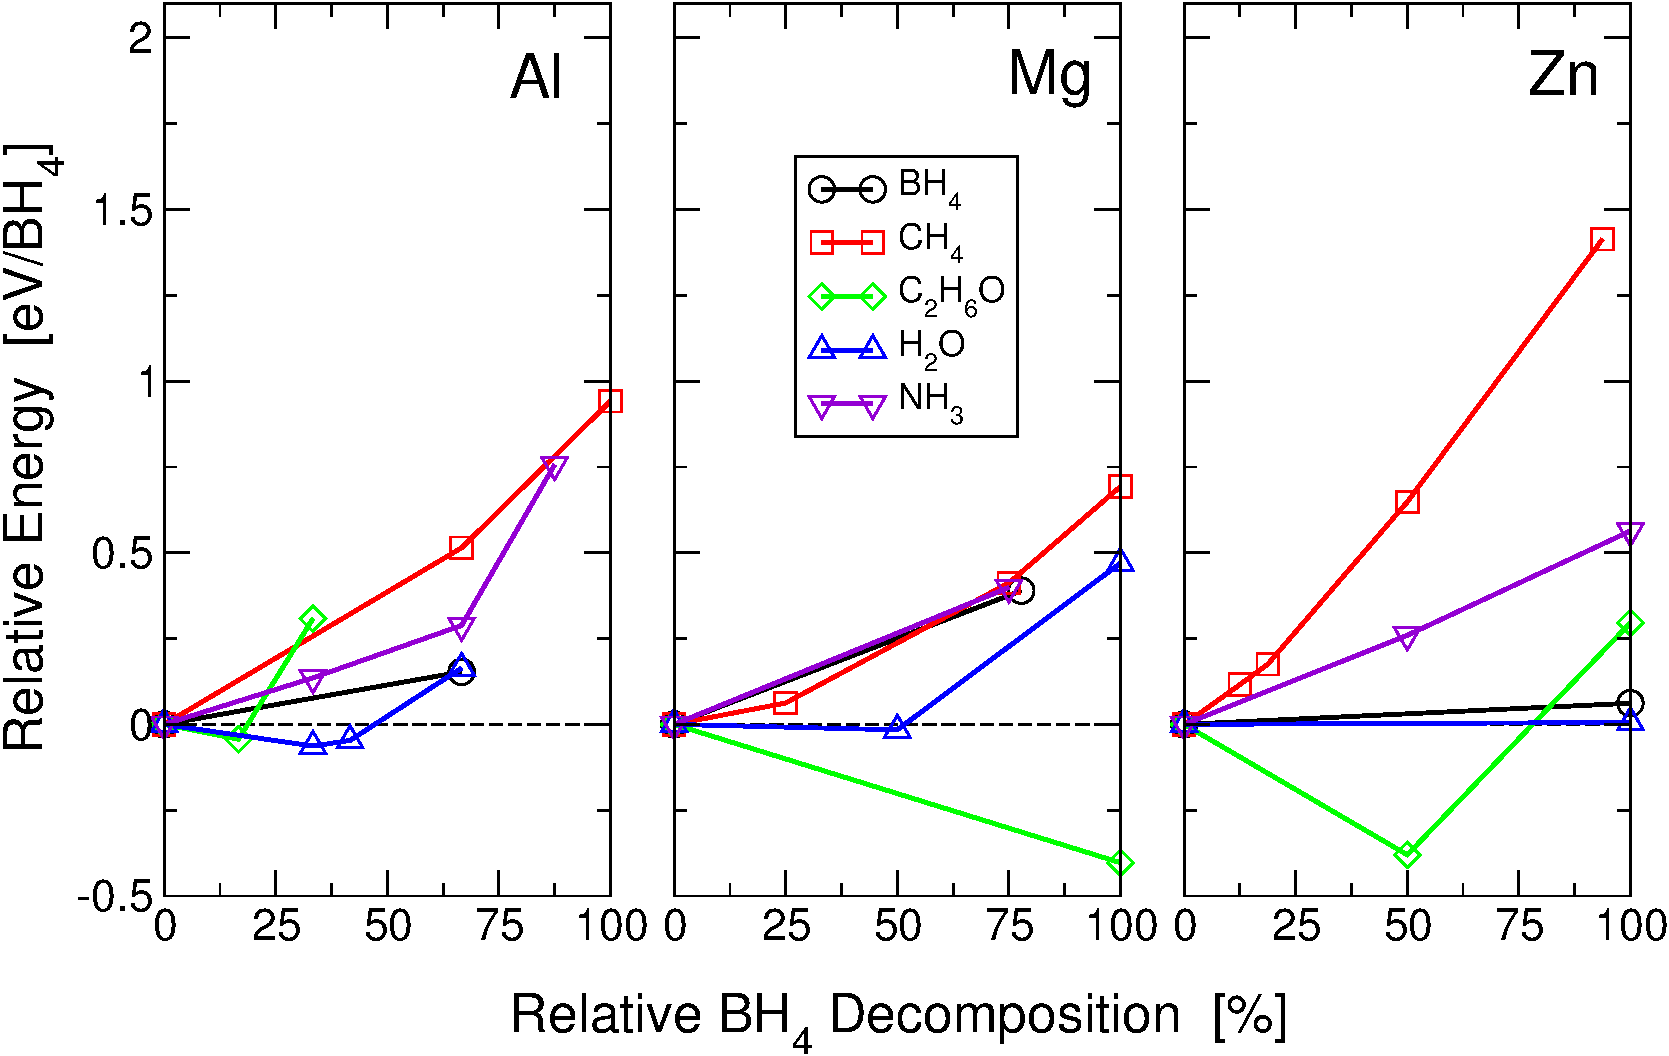
\includegraphics[width=\columnwidth]{BH4_decomposition}
\caption{\label{fig:boro_decom}Plot of energy vs.\ relative BH$_4$ decomposition for all structures
found in structure search
lying along the bottom hull for Al(BH$_4$)$_3$, Mg(BH$_4$)$_2$, and 
Zn(BH$_4$)$_2$, and their corresponding additive molecules. `BH$_4$' on the plot legend indicates the pure
borohydride, i.e.\ no additive.}
\end{figure}


\begin{figure}
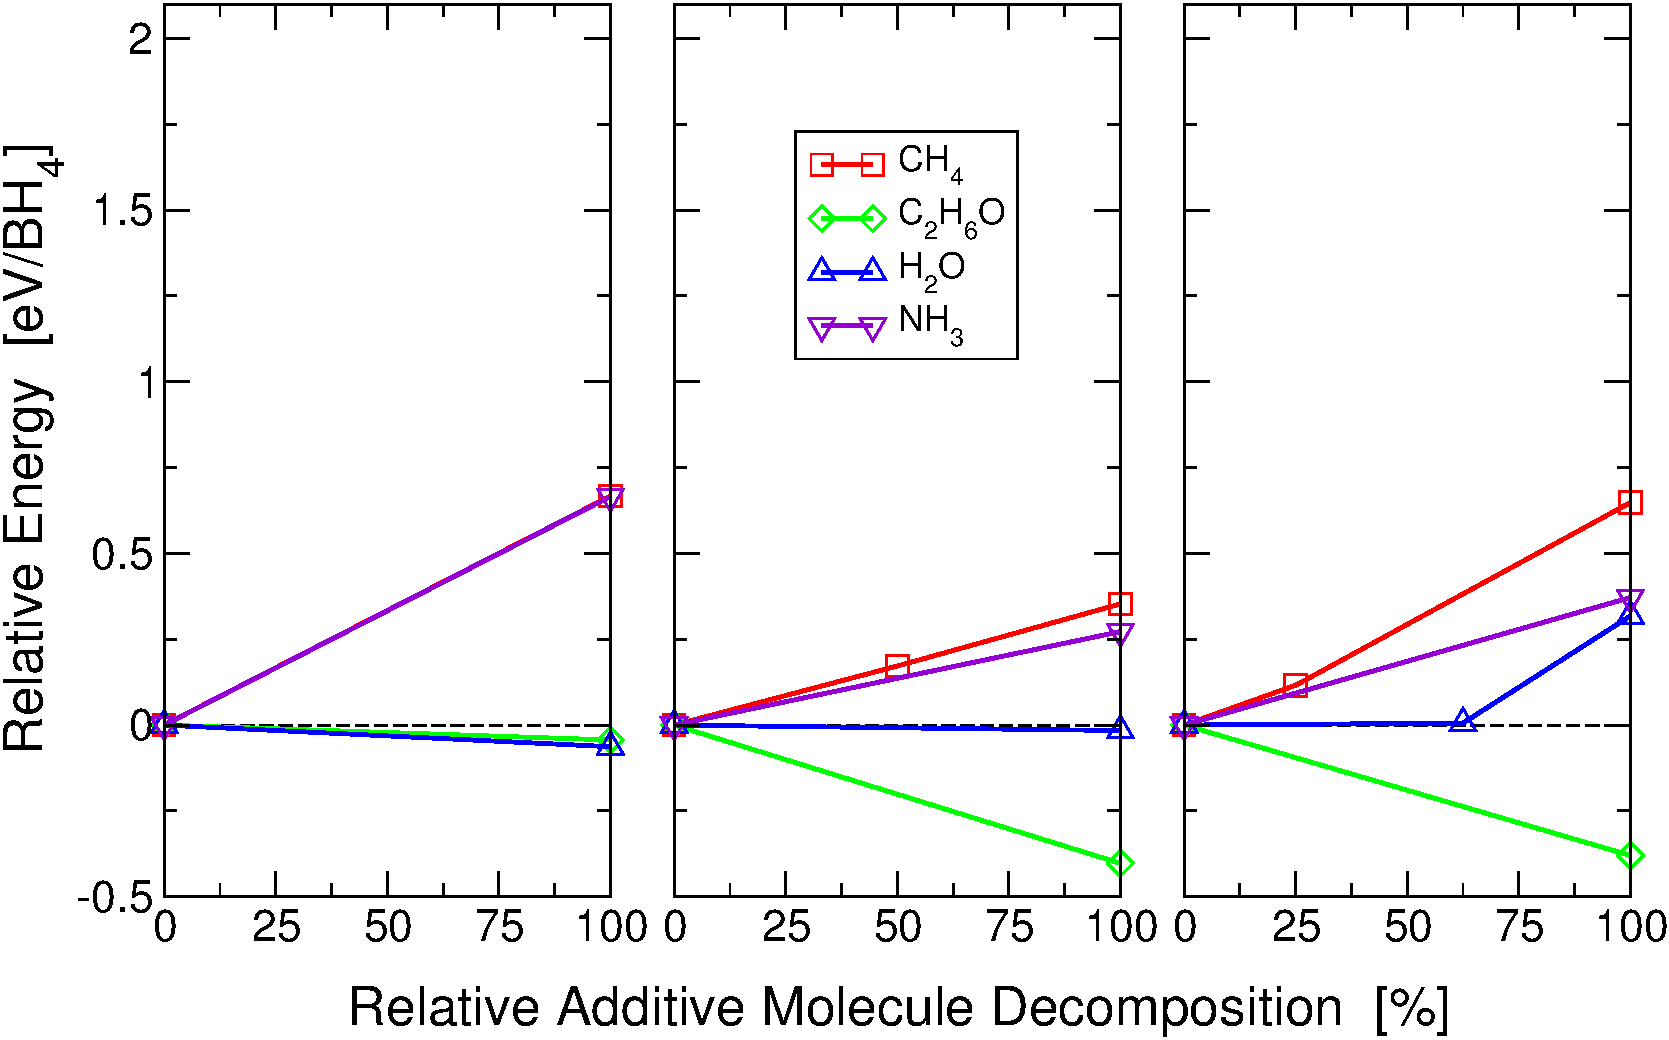
\includegraphics[width=\columnwidth]{molecule_decomposition}
\caption{\label{fig:add_decom}Plot of energy vs.\ relative additive molecule decomposition for all structures
found in structure search
lying along the bottom hull for Al(BH$_4$)$_3$, Mg(BH$_4$)$_2$, and 
Zn(BH$_4$)$_2$, and their corresponding additive molecules.}
\end{figure}

As on overview to understanding Fig.~\ref{fig:main_plot}, notice first the general trend that structures
which contain more H$_2$ have, with a few exceptions, a higher relative energy. This is to be expected; it takes
energy to release the hydrogen molecules. However, it is interesting to note that the curves seem to concave upward, meaning
that the initial hydrogen release seems to hinder, rather than facilitate, additional hydrogen release.
Further notice that the maximum amount of H$_2$ produced seems to vary depending on both the 
particular borohydride and additive used, a point which will be discussed further in the following paragraphs. Finally, notice that,
in exception to the general trend, certain structures seem to decrease in relative energy, signifying at the very least
that the initial structure is a metastable state.

It should be noted that while many total structures were analyzed via
the evolutionary metadynamics technique, for certain combinations of
borohydrides and additives relatively few concentrations of H$_2$ were
obtained.  For example, for unaltered Al(BH$_4$)$_3$, only two non-zero
concentrations of H$_2$ were found, only one of which lay on the convex hull,
leading to a total of only two data points for this structure in
Fig.~\ref{fig:main_plot}.  This is likely due to the relative difficulty to
produce H$_2$ molecules in Al(BH$_4$)$_3$, as seen by its relatively low H$_2$
production in experiment (see Fig.~6 from reference \cite{Nakamori_2007:thermodynamical_stabilities}).

As the maximum concentration of a given molecule seen corresponds roughly to
the maximum concentration of that molecule in nearby metastable states, we
would also expect the maximum concentration to correlate with how much of that
molecule is produced during the decomposition process.  In fact, comparing
again with experimental thermal decomposition data for Al(BH$_4$)$_3$,
Mg(BH$_4$)$_2$, and Zn(BH$_4$)$_2$, we find that the relative ordering of
maximum hydrogen concentration we found corresponds to the relative experimental
hydrogen production (to wit, from least to greatest production, Al, Mg, and
then Zn(BH$_4$)$_2$) \cite{Nakamori_2006:correlation_between, Nakamori_2007:thermodynamical_stabilities}. Further
supporting this hypothesis that the maximum concentration of H$_2$ produced
corresponds with the amount that would be produced in experiment is that the
amount of H$_2$ produced in Mg(BH$_4$)$_2$ is substantially increased when
complexed with
NH$_3$\cite{Soloveichik_2008:ammine_magnesium}, which
agrees qualitatively with the increase in maximum hydrogen concentration seen
in Mg(BH$_4$)$_2$$\cdot$NH$_3$. Another piece of evidence is that the same relative
trends are seen for certain additives and certain metals (e.g.\ CH$_4$ is
always found to have the highest H$_2$ concentration).  However, it should be
pointed out that, as most of the proposed materials haven't been studied
experimentally, it is difficult to ascertain just how valid drawing inferences
from these plots can be.


\subsubsection{Analysis of y-axis}

Looking now at the relative energy costs for producing H$_2$, i.e. the y-axis
of the plots, we see results that we would more or less expect. Notably, for
Mg(BH$_4$)$_2$ we see that there is a significant decrease in the energy cost
to produce H$_2$ when there is an additive molecule involved, regardless of
which particular molecule it is. This is unsurprising, as it is known
experimentally that complexing
Mg(BH$_4$)$_2$ with NH$_3$ significantly decreases
the temperature of hydrogen release\cite{Soloveichik_2008:ammine_magnesium}, so it is
plausible that complexing with other additives has a similar effect.  For
Al(BH$_4$)$_3$ and Zn(BH$_4$)$_2$, we see the effects of additive molecules are
much less pronounced, with e.g.\ NH$_3$ seeming to have approximately the same cost in energy to
producing H$_2$; this also agrees with experimental results which find that
although Al(BH$_4$)$_3$$\cdot2$NH$_3$ evolves more H$_2$ than the pure borohydride,
the temperature of hydrogen release is approximately the
same\cite{Guo_2012:ammine_aluminium}.  It also agrees with the
overall trend that NH$_3$ tends to destabilize stable borohydrides (i.e.\
Mg(BH$_4$)$_2$) while stabilizing unstable borohydrides (i.e.\ Zn(BH$_4$)$_2$
and Al(BH$_4$)$_3$)\cite{Soloveichik_2008:ammine_magnesium}.  It should be noted here that
in comparisons to experimental results on ammine borohydrides, in many cases
studies were done on materials with 2 or 3 NH$_3$ units per formula unit, whereas in all of our
complexes there was one additive molecule per formula unit; we argue that while
the properties of the material depend upon the concentration of NH$_3$ (e.g.\ the temperature
of hydrogen release tends to increase with the number of NH$_3$ units), the
most significant factor qualitatively is whether or not the material has been
complexed with NH$_3$ at all (e.g.\ see this study done on ammine
aluminum borohydride with varying concentrations of NH$_3$)\cite{Guo_2012:ammine_aluminium}.

Looking specifically at the case of pure borohydrides, one surprising result is that Al(BH$_4$)$_3$ seems to have a higher barrier
to H$_2$ production than Zn(BH$_4$)$_2$, whereas experimentally Al(BH$_4$)$_3$
releases hydrogen at a lower temperature (330K compared to 410K)\cite{Nakamori_2007:thermodynamical_stabilities}. There are
two explanations we offer for this. The first is that it is helpful to remember
that the points on the plots we present are local minima, so don't necessarily fully capture the energy
barrier for transitioning from one state to the next (although in general as an approximation
we are assuming the Bell--Evans--Polanyi principle to hold true); it is possible that 
the kinetic barrier for transitioning between states is significantly larger for
Zn(BH$_4$)$_2$ than for Al(BH$_4$)$_3$. The second explanation is that the
energy barrier for the diffusion of H$_2$ molecules to escape the bulk is 
higher for Zn(BH$_4$)$_2$. We find this plausible due to the fact that, unlike most borohydrides,
Al(BH$_4$)$_3$ is known to be a liquid at ambient temperatures.
Finally, it should be noted that our results for the relative ordering of barrier to H$_2$
production also agree with the known thermodynamic stabilities of Zn(BH$_4$)$_2$,
Al(BH$_4$)$_3$, and Mg(BH$_4$)$_2$, so they are in fact not so surprising; it simply
seems that there is a kinetic factor causing Al(BH$_4$)$_3$ to release H$_2$ at a
lower temperature than Zn(BH$_4$)$_2$.


Continuing now to examine the case with additive molecules, it mostly seems that they
have similar effects on the barrier to H$_2$ production, with the relative
ordering among them differing upon which concentration and which borohydride 
is looked at. One noticeable trend is that H$_2$O, which seems to have a 
noticeably lower barrier to H$_2$ production than other additives. 

The physical reasoning for the trends seen here is somewhat of a mystery.
For example, we had initially expected H$_2$O to behave most similarly to
NH$_3$ (in Figs.~\ref{fig:main_plot}--\ref{fig:add_decom}) due to it also being a small, polar molecule.
However, we see in fact that CH$_4$ behaves most similarly to NH$_3$, despite being a nonpolar
molecule. The relatively low energy required to produce H$_2$ for borohydrides complexed
with H$_2$O could be due to the willingness of H$_2$O to react with the BH$_4$ unit, 
as we see that it commonly forms BH$_3$-OH or BH$_2$-OH, leaving behind spare hydrogens to produce H$_2$.
However, it is still difficult to say for sure why this mechanism for producing hydrogen should have
noticeably lower barriers than similar mechanisms for other additives. Ultimately, while it 
would have been desirable to be able to determine general rules in order to predict
the effects of additives, we found this to be beyond the scope of this work (and in fact,
explaining the physical mechanism behind one given additive may not be very illuminating
in general). Instead, we study the effects of 4 specific additives and provide a computational
method for determining the effects of other possible additives.

\subsubsection{Analysis of BH$_4$ and additive decomposition}

To gain further insight we also plot here the relative energy cost to decompose
the BH$_4$ units in Fig.~\ref{fig:boro_decom} and the relative energy cost to 
decompose the additive molecules in Fig.~\ref{fig:add_decom} (note that for easy comparison all three figures
have the same y-axis scaling). The meaning of the y-axis for these plots is comparable to that in Fig.~\ref{fig:main_plot},
except that it is for molecule decomposition instead of formation (e.g.\ 75\% relative decomposition of BH$_4$ in a $2\times2\times2$
supercell of Al(BH$_4$)$_3$ would correspond to 6 BH$_4$ molecules found). 

The primary use of Figs.~\ref{fig:boro_decom} and \ref{fig:add_decom} is to provide additional information and context
to understanding the decomposition and hydrogen release processes for the various structures. We would hope that,
ideally, Figs.~\ref{fig:main_plot} and \ref{fig:boro_decom} would be closely related, i.e.\ an increase in BH$_4$ decomposition
ought to lead to additional H$_2$ formation, and ideally the two would have similar energy profiles. As an example, compare the cases
of Figs.~\ref{fig:boro_decom} and \ref{fig:add_decom} for Mg(BH$_4$)$_2\cdot$C$_2$H$_6$O: we see clearly an increase
in relative energy along the lowest-energy path to produce H$_2$, but we see a decrease in relative energy to decompose BH$_4$. It would seem in this case, the most favorable path for Mg(BH$_4$)$_2\cdot$C$_2$H$_6$O is to decompose BH$_4$ (and, in fact, also
C$_2$H$_6$O itself looking at Fig.~\ref{fig:add_decom}), providing some evidence that Mg(BH$_4$)$_2\cdot$C$_2$H$_6$O
may be a poor hydrogen storage candidate, due to its unwillingness to release H$_2$ compared to its willingness to
decompose. In other words, it is desirable for the curves in Figs.~\ref{fig:boro_decom} and \ref{fig:add_decom} to have
energies not significnatly lower than those found in Fig.~\ref{fig:main_plot}. 

It should now be noted in general that there are clearly certain combinations of additives and concentrations
which result in a negative energy relative to the starting structure. This clearly indicates that in these instances,
the starting structure was, to a greater or lesser extent, a metastable structure, and that a more favorable
configuration could be obtained via molecule reactions.

Looking at the energy cost to decompose the BH$_4$ units, it's clear that
for the pure borohydrides, the energy cost to decompose BH$_4$ shows a clear
correlation with the thermodynamic stability of the material, with pure Zn(BH$_4$)$_2$
having almost no thermodynamic barrier to BH$_4$ decomposition. 
For the case of additives, it seems that NH$_3$ and CH$_4$ seem to have a stabilizing
effect while H$_2$O and C$_2$H$_6$O seem to have a destabilizing effect. Furthermore,
it seems the relative stabilization/destabilization corresponds roughly to the stability of
the borohydride, with Mg(BH$_4$)$_2$ seeing anywhere from no stabilization to significant
destabilization, whereas the less stable Al(BH$_4$)$_3$ and Zn(BH$_4$)$_2$ seeing
anywhere from significant stabilization to minor destabilization.

This trend in NH$_3$ and CH$_4$ stabilizing the material and H$_2$O and C$_2$H$_6$O
destabilizing material is more understandable when looking at the energy costs
to decompose these molecules. Whereas NH$_3$ and CH$_4$ always have relatively
high, positive barriers to decomposition, H$_2$O and C$_2$H$_6$O have (with one exception) consistently
negative barriers to decomposition. In fact, looking at H$_2$O and C$_2$H$_6$O
across all plots we see that they often have negative or near-zero energy
differences with respect to their starting structures, meaning that in many
cases the structure would prefer to transition to a more energetically favorable
state by having its molecular constituents react with one another. Looking in 
detail at some of the most favorable structures for these additives, we find
that in general this involves (not surprisingly) the additive molecule reacting
with the BH$_4$ unit; for example in Mg(BH$_4$)$_2$$\cdot$H$_2$O, we found the 
most favorable structure involved the reaction of H$_2$O and a single
BH$_4$ molecule to form H$_4$BO and H$_2$. 

\subsubsection{Summary of results}

Synthesizing and summarizing our thermodynamic and metadynamics results,
it seems that how a borohydride will respond to additives depends on where
it falls along the ``stability line'', a well-known phenemenon related
to a borohydride's metal's electronegativity (and in fact, as we show in our
recent paper, more accurately described by its formation enthalpy) \cite{Harrison_2016:suppressing_diborane}, wherein
borohydrides to the right of the stability line are known to not produce
diborane and have their temperature of hydrogen release lowered when complexed
with NH$_3$, whereas borohydrides to the left of the stability line are
known to produce diborane and are generally known to have their temperature
of hydrogen release increased when complexed with NH$_3$. More stable borohydrides
are less willing thermodynamically to be complexed with additives, but see
a more pronounced effect in the amount of H$_2$ produced, whereas in less
stable borohydrides, additives tend to suppress the production of unwanted
byproducts (i.e.\ B$_2$H$_6$) by stabilizing the material, although they
do not see as impressive results in lowering the hydrogen release temperature.


One of the most promising specific findings of this study is that out of the
small molecules we studied, while most seem to have effects comparable to 
NH$_3$, H$_2$O in particular seems to have a significantly lower reaction
pathway to produce H$_2$ when complexed with borohydrides. 
Another promising candidate is CH$_4$, which seems to have very similar
effects to NH$_3$ looking at Figs.~\ref{fig:main_plot}--\ref{fig:add_decom},
although it consistently evolves more H$_2$ as seen if Fig.~\ref{fig:main_plot}.
It is interesting to note that while the success of NH$_3$ as an additive is thought
to be largely due to its polarity\cite{Guo_2012:ammine_aluminium,Welchman_2017:decomposition_mechanisms}, CH$_4$
sees similar results here despite the fact that it is nonpolar. While we
would want to see experimental verification to corroborate this result,
it is possible that the polarity of the additive molecule is not wholly
descriptive of its effect.

However, it should
be mentioned that, for the three new potential additive molecules studied, it is unknown
how feasible forming a stable borohydride structure would be, as
seen by either their thermodynamic stability in Fig.~\ref{fig:reaction_enthalpies} (especially for CH$_4$), the
fact that some of their structures see a decrease in energy as BH$_4$ is decomposed
as seen in Fig.~\ref{fig:boro_decom}, or the fact that structures tend to
decrease in energy as the additive molecule is decomposed as seen in Fig.~\ref{fig:add_decom}.
However, it may be that these structures formed from a borohydride-additive complex, although not strictly borohydrides
once the BH$_4$ reacts with the additive molecule, are themselves very good hydrogen storage materials,
as evidenced by their low-energy pathways to release H$_2$.


Perhaps most promising in general is that the method we've employed here---
that is, using evolutionary metadynamics to study the local metastable
states of a system combined with a structure search to provide the initial
starting structures---has produced results that are both internally consistent
and consistent with previous experimental and theoretical studies (inasmuch as
there exists other studies which can be compared to). We see that this
technique would prove very useful for any instance where the effects
of additives (or indeed, other structural modifications) on the possible
reaction pathways of a given system is desired.


%%%%%%%%%%%%%%%%%%%%%%%%%%%%%%%%%%%%%%%%%%%%%%%%%%%%%%%%%%%%%%%%%%%%%%%%
\section{Conclusions}
%%%%%%%%%%%%%%%%%%%%%%%%%%%%%%%%%%%%%%%%%%%%%%%%%%%%%%%%%%%%%%%%%%%%%%%%


The thermodynamic properties and local metastable states were investigated
for 15 total structures, which included all combinations of 3 representative borohydrides
complexed with 4 possible additive molecules (including no additive). 
Although it is unfortunately unfeasible to fully simulate the borohydride decomposition reaction,
we find that our results on local metastable states correlate well with experimental results
for the full decomposition reaction, indicating that the initial steps in decomposition
partially dictate the full decomposition reaction. Further, we find that the energy
differences we see between metastable states and initial ground-state structure
agree closely with previous NEB calculations (where comparisons could be made),
indicating that the Bell--Evans--Polanyi principle seems to hold true.
Although we are reluctant to be overly confident without experimental verification,
our results indicate that additives other than NH$_3$ could see similarly
impressive results in improving the hydrogen-storage properties of borohydrides,
particularly H$_2$O. Finally, we believe more generally that the
techniques used in this investigation, particularly evolutionary metadynamics,
would be very helpful in future studies seeking to ascertain the effects
on structural changes to chemical reactions, especially those where the reaction
is relatively simple (e.g.\ simple diffusion).




\section*{Acknowledgements}
This work was supported in full by NSF Grant No.\ DMR--1145968.

\section*{Appendix--Overview of evolutionary metadynamics}
Since the evolutionary metadynamics method is fairly new, we provide
here a summary---further detail can be found in the relevant literature, with previous examples including
finding high-pressure carbon allotropes, multiple boron configurations and phase transition pathways, and stable and metastable states for a 
variety of silicon-containing compounds.
\cite{Zhu_2012:systematic_search,Zhu_2012:evolutionary_metadynamics,Zhu_2015:generalized_evolutionary}.
This technique allows for a sampling of rare events by adding cumulative Gaussian energy penalties to regions of phase space that have already been explored.
However, care must be taken when choosing these so-called \emph{collective variables},
i.e.\ the variables to which an energy penalty is added. One well-known technique
for sampling nearby metastable states for a known stable structure is to use the unit cell's
size and shape as the collective variables and then using molecular dynamics (e.g.\ simulated annealing)
in order to determine the atomic positions \cite{Marto-n-nak_2003:predicting_crystal}. However, this method can result
in highly disordered systems \cite{Zhu_2015:generalized_evolutionary}. Recently, it has been found that when metadynamics
is combined with an evolutionary algorithm typically seen in crystal structure
prediction techniques, it is possible to generate many nearby metastable states
to a given initial structure \cite{Zhu_2012:evolutionary_metadynamics,Zhu_2015:generalized_evolutionary}. While metadynamics has been developed
over a
decade ago \cite{Laio_2002:escaping_free-energy}, this approach is still relatively new. The method then proceeds as follows: The user
provides a reference structure (ideally the ground-state structure) and the 
Gaussian height and width. Then, the vibrational eigenvectors and corresponding frequencies
are solved for, providing a means to perturb the system, with the magnitude of the perturbation
dependent on the chosen Gaussian height and width; the idea is that low activation barriers
are expected to be in the direction of the lowest curvature of the free-energy landscape (i.e.\
the softest vibrational modes). In summary, by combining \textsc{Uspex}'s evolutionary algorithm with metadynamics and using
constrained variables inspired by the dynamical matrix of the ground-state structure, it is possible to sample
many nearby low-energy metastable states.


\section*{References}
%%%%%%%%%%%%%%%%%%%%%%%%%%%%%%%%%%%%%%%%%%%%%%%%%%%%%%%%%%%%%%%%%%%%%%%%
\bibliography{compiled}
%%%%%%%%%%%%%%%%%%%%%%%%%%%%%%%%%%%%%%%%%%%%%%%%%%%%%%%%%%%%%%%%%%%%%%%%




%%%%%%%%%%%%%%%%%%%%%%%%%%%%%%%%%%%%%%%%%%%%%%%%%%%%%%%%%%%%%%%%%%%%%%%%
\end{document}
%%%%%%%%%%%%%%%%%%%%%%%%%%%%%%%%%%%%%%%%%%%%%%%%%%%%%%%%%%%%%%%%%%%%%%%%
